\chapter{Evaluation}
\label{cha:evaluation}

\section{No Trailer, Generation Count of 50}
\label{sec:no_trailer_50}

In the following chapter we will compare the results, that is the path rating, and the required computation time for several different versions of the genetic algorithm.
Since there are many values and functions within the GA that can be adjusted and influence its performance, only a few can be considered here. The conclusion drawn in the next chapter \ref{cha:conclusion} will be based on the evaluation here.

The following table shows the rating achieved (higher is better) as well as the time needed for computation (lower is better) for several different setups of the algorithm. For each setup 7 runs and an average is given. Only the choice in GA functions used is changed between different runs, the remaining settings are consistent throughout the table and are as follows.

The population size is 1000, the algorithm runs for 50 generations and has a crossover rate of 60\%, a mutation rate of 0.1\% and without reordering operation. It starts at 175,350 and the destination is 740,100 (both are the program's default values). The vehicle has no trailers, an M value of 24,55, an L value of 42,5, and a starangle of 45°, these values have been randomly generated and were then kept throughout all test runs.
Computation was done on a Core2Quad 6600@2.4GHz with 4GB of System Memory.

\begin{center}
	\begin{tabular}{| l | l | l | p{3cm} | p{3cm}|}
		\hline
		Run 		& 8Bit, Tournament 	& 8Bit, Roulette 	& TwoPoint, Tournament 	& TwoPoint, Roulette	\\ \hline
		1				&	152 in 1:50				&	222 in 1:44			&	647 in 1:53						&	49 in 1:57					\\ \hline
		2				&	90 in 1:47				&	134 in 1:51			& 111 in 154 \ref{pic:example_good_path}			&	127 in 2:01 \ref{pic:example_problem_path}	\\ \hline		
		3				&	127 in 1:48				&	106 in 1:54			& 240 in 1:48						& 51 in 1:58					\\ \hline
		4				&	240 in :144				&	61 in 1:46			& 122 in 1:48						& 130 in 2:01					\\ \hline
		5				&	152 in 1:49				&	222 in 1:57			&	274 in 1:49						&	156 in 1:54					\\ \hline
		6				&	163 in 1:49				& 201 in 1:56			&	56 in 1:57						& 78 in 1:51					\\ \hline
		7				&	90 in 2:06				&	76 in 1:53			& 59 in 1:47						& 230 in 1:56					\\ \hline
		Best		&	240 in 1:44				&	222 in 1:44			&	647 in 1:53						&	156 in 1:54					\\ \hline
		Worst		&	90 in 2:06				&	61 in 1:46			&	56 in 1:57						& 49 in 1:57					\\ \hline
		Average	&	144 in 1:51				& 146 in 1:51			& 198 in 1:50						&	117 in 1:56					\\ \hline
		\hline
	\end{tabular}
\end{center}


As can be seen from these results, the time is relatively consistent at just below 2 minutes. This of course depends heavily on the hardware used, but surprisingly very little on the oprations chosen within the GA. The results are not quite as consistent and have to be handled carefully due to the small sample size. Row 3 (TowPointCrossover, TournamentSelection) seems to deliver the best result, but this is largely due to a single very good path, which can be attributed to "`luck"' in the random generated phase. If we disregard this single path we get an average of 143, which is almost the same as in the first two rows. The last row (TwoPointCrossover, RouletteWheelSelection) however produced sub-optimal paths rather consistently. It is also noticable that the difference between the best and worst path is much smaller in the first row when compared to the other three, which is why this setting has been chosen as the default one as it produces an acceptzable quality of paths rather consitently. These results may of course change with a (much) larger sample sizes.
The overall quality of the paths is rather low, which we will try to mitigate by raising the generation count in the next test, the real cause for this however is probably the rather primitive fitness function, see \ref{cha:conclusion} for further discussion. Right now the algorithm depends rather heavily on its initial random paths which leads to very different and overall sub-optimal results.
Two interesting paths are given in fig. \ref{pic:example_good_path} and fig. \ref{pic:example_problem_path}. Here, red is the path planned by the GA and blue is the actual, driveable, path obtained via simulation. In fig \ref{pic:example_good_path} we see an example of a good path which avoids all obstacles and gets very close to the target position. Whether or not it also hits the target configuration is not considered by the current fitness function. The path got a rating of 111, which is rather low compared to the ratings of some of the other, objectively worse, paths, which also points to the fitness function as the algorithms current weakness. \ref{pic:example_problem_path} shows a different problem with the current evaluation as it shows a path with a good rating (127) which also seems fine for the most part, but is completely impossible in reality as it passes through a wall. The current collision detection gives a worse rating the "`longer"' the path stays within the black area, which means that crossing a thin wall like this doesn't lower the rating by a whole lot compared to the positive rating it receives from the distance evaluation, even though the path is obvisouly still unusable. The current evaluation emphasizes distance to the target over the collision detection in order to obtain more acceptable paths quickly, but further optimization is required to make sure this does not come at the cost of accepting impossible paths.

\begin{figure}[h]
\centering
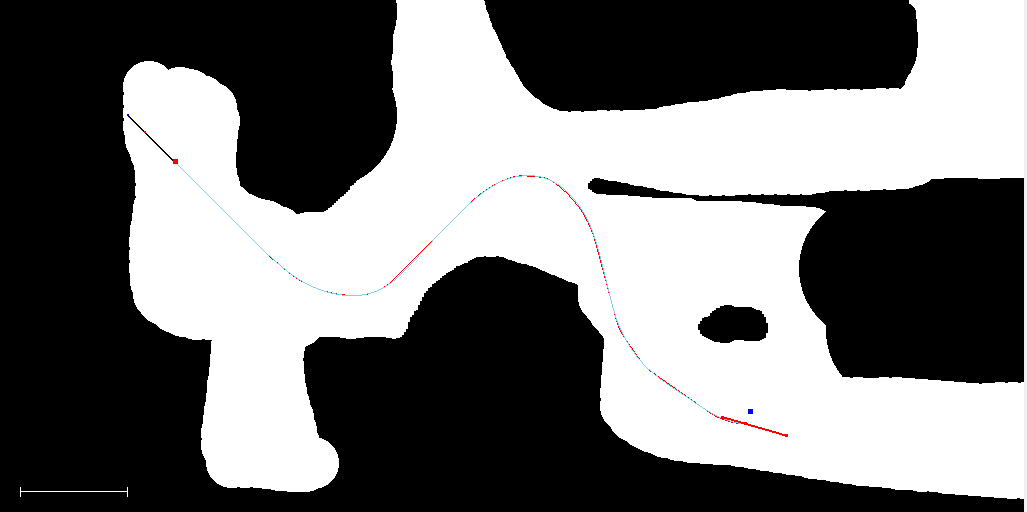
\includegraphics[width=0.75\textwidth]{./Chapters/Figures/example_good_path.png}
\caption{Example of a good result computed by the GA\label{pic:example_good_path}}
\end{figure}

\begin{figure}[h]
\centering
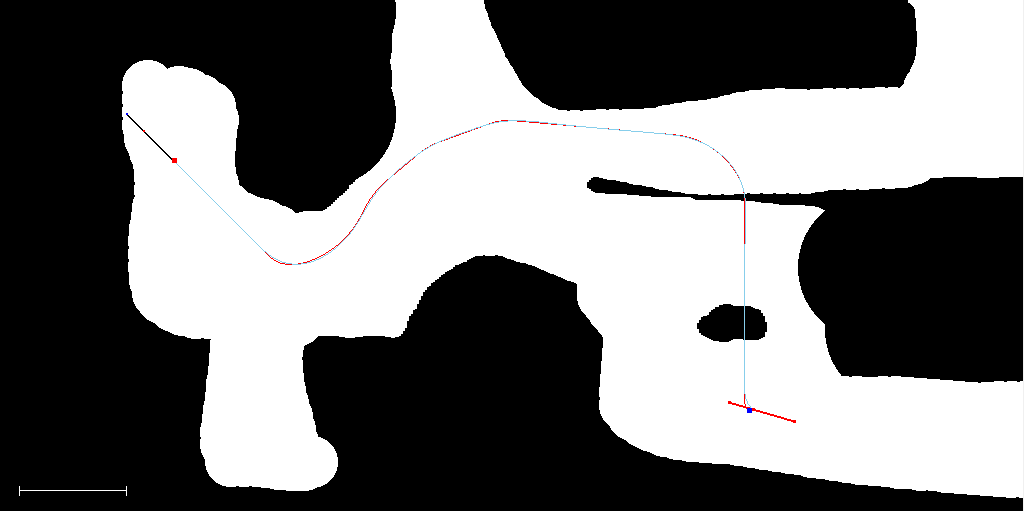
\includegraphics[width=0.75\textwidth]{./Chapters/Figures/example_problem_path.png}
\caption{A bad path with a good rating produced by the GA\label{pic:example_problem_path}}
\end{figure}

\section{No Trailer, Generation Count of 100}
\label{sec:no_trailer_100}

The settings in the following table are the exact same as in the previous ones, but the generation count has doubled to 100.

\begin{center}
	\begin{tabular}{| l | l | l | p{3cm} | p{3cm}|}
		\hline
		Run 		& 8Bit, Tournament 	& 8Bit, Roulette 	& TwoPoint, Tournament 	& TwoPoint, Roulette	\\ \hline
		1				&	152 in 1:50				&	222 in 1:44			&	647 in 1:53						&	49 in 1:57					\\ \hline
		2				&	90 in 1:47				&	134 in 1:51			& 111 in 154 \ref{pic:example_good_path}			&	127 in 2:01 \ref{pic:example_problem_path}	\\ \hline		
		3				&	127 in 1:48				&	106 in 1:54			& 240 in 1:48						& 51 in 1:58					\\ \hline
		4				&	240 in :144				&	61 in 1:46			& 122 in 1:48						& 130 in 2:01					\\ \hline
		5				&	152 in 1:49				&	222 in 1:57			&	274 in 1:49						&	156 in 1:54					\\ \hline
		6				&	163 in 1:49				& 201 in 1:56			&	56 in 1:57						& 78 in 1:51					\\ \hline
		7				&	90 in 2:06				&	76 in 1:53			& 59 in 1:47						& 230 in 1:56					\\ \hline
		Best		&	240 in 1:44				&	222 in 1:44			&	647 in 1:53						&	156 in 1:54					\\ \hline
		Worst		&	90 in 2:06				&	61 in 1:46			&	56 in 1:57						& 49 in 1:57					\\ \hline
		Average	&	144 in 1:51				& 146 in 1:51			& 198 in 1:50						&	117 in 1:56					\\ \hline
		\hline
	\end{tabular}
\end{center}

\section{One Trailer, Generation Count of 50}
\label{sec:no_trailer_50}

The settings in the following table are the exact same as in the previous ones, excpet that the vehicle now has one trailer and the generation count is lowered to 50 again.

\begin{center}
	\begin{tabular}{| l | l | l | p{3cm} | p{3cm}|}
		\hline
		Run 		& 8Bit, Tournament 	& 8Bit, Roulette 	& TwoPoint, Tournament 	& TwoPoint, Roulette	\\ \hline
		1				&	152 in 1:50				&	222 in 1:44			&	647 in 1:53						&	49 in 1:57					\\ \hline
		2				&	90 in 1:47				&	134 in 1:51			& 111 in 154 \ref{pic:example_good_path}			&	127 in 2:01 \ref{pic:example_problem_path}	\\ \hline		
		3				&	127 in 1:48				&	106 in 1:54			& 240 in 1:48						& 51 in 1:58					\\ \hline
		4				&	240 in :144				&	61 in 1:46			& 122 in 1:48						& 130 in 2:01					\\ \hline
		5				&	152 in 1:49				&	222 in 1:57			&	274 in 1:49						&	156 in 1:54					\\ \hline
		6				&	163 in 1:49				& 201 in 1:56			&	56 in 1:57						& 78 in 1:51					\\ \hline
		7				&	90 in 2:06				&	76 in 1:53			& 59 in 1:47						& 230 in 1:56					\\ \hline
		Best		&	240 in 1:44				&	222 in 1:44			&	647 in 1:53						&	156 in 1:54					\\ \hline
		Worst		&	90 in 2:06				&	61 in 1:46			&	56 in 1:57						& 49 in 1:57					\\ \hline
		Average	&	144 in 1:51				& 146 in 1:51			& 198 in 1:50						&	117 in 1:56					\\ \hline
		\hline
	\end{tabular}
\end{center}

\section{One Trailer, Generation Count of 100}
\label{sec:no_trailer_100}

The settings in the following table are the exact same as in the previous ones, but the generation count has doubled to 100 again. The vehicle still has one trailer.

\begin{center}
	\begin{tabular}{| l | l | l | p{3cm} | p{3cm}|}
		\hline
		Run 		& 8Bit, Tournament 	& 8Bit, Roulette 	& TwoPoint, Tournament 	& TwoPoint, Roulette	\\ \hline
		1				&	152 in 1:50				&	222 in 1:44			&	647 in 1:53						&	49 in 1:57					\\ \hline
		2				&	90 in 1:47				&	134 in 1:51			& 111 in 154 \ref{pic:example_good_path}			&	127 in 2:01 \ref{pic:example_problem_path}	\\ \hline		
		3				&	127 in 1:48				&	106 in 1:54			& 240 in 1:48						& 51 in 1:58					\\ \hline
		4				&	240 in :144				&	61 in 1:46			& 122 in 1:48						& 130 in 2:01					\\ \hline
		5				&	152 in 1:49				&	222 in 1:57			&	274 in 1:49						&	156 in 1:54					\\ \hline
		6				&	163 in 1:49				& 201 in 1:56			&	56 in 1:57						& 78 in 1:51					\\ \hline
		7				&	90 in 2:06				&	76 in 1:53			& 59 in 1:47						& 230 in 1:56					\\ \hline
		Best		&	240 in 1:44				&	222 in 1:44			&	647 in 1:53						&	156 in 1:54					\\ \hline
		Worst		&	90 in 2:06				&	61 in 1:46			&	56 in 1:57						& 49 in 1:57					\\ \hline
		Average	&	144 in 1:51				& 146 in 1:51			& 198 in 1:50						&	117 in 1:56					\\ \hline
		\hline
	\end{tabular}
\end{center}